\documentclass[11pt,a4paper]{article}
\usepackage[margin=18mm]{geometry}
\usepackage{amsmath,amssymb,mathtools}
\usepackage{booktabs,array,enumitem}
\usepackage[dvipsnames]{xcolor}
\usepackage{graphicx,listings,tikz,needspace}
\usetikzlibrary{arrows.meta,positioning}
\usepackage[most]{tcolorbox}
\usepackage{hyperref}
\hypersetup{colorlinks=true,urlcolor=MidnightBlue,linkcolor=MidnightBlue}
\setlength{\parindent}{0pt}\setlength{\parskip}{4pt}
\newcommand{\course}{PHY4605 Computational Methods in Physics}
\newcommand{\units}[1]{\,\mathrm{#1}}
\newtcolorbox{keybox}{colback=RoyalBlue!5,colframe=RoyalBlue!65!black,boxrule=.7pt,arc=2mm}
\newtcolorbox{checkbox}{colback=ForestGreen!5,colframe=ForestGreen!55!black,boxrule=.7pt,arc=2mm}
\newtcolorbox{aibox}{colback=BurntOrange!7,colframe=BurntOrange!80!black,boxrule=.7pt,arc=2mm}
\lstdefinestyle{matlabstyle}{language=Matlab,basicstyle=\ttfamily\footnotesize,keywordstyle=\color{RoyalBlue!75!black},commentstyle=\color{ForestGreen!55!black},stringstyle=\color{BurntOrange!80!black},numbers=left,numberstyle=\scriptsize\color{black!50},numbersep=5pt,frame=single,rulecolor=\color{RoyalBlue!25},backgroundcolor=\color{RoyalBlue!3},showstringspaces=false,columns=fullflexible,keepspaces=true,breaklines=true}
\begin{document}
{\large\textsc{\course}}\\[-2pt]
{\small Learning Note \textbar\ Week 13}\par\vspace{4pt}
{\LARGE\bfseries Computational Investigation: Present, defend, and hand off a validated physical model}\par\vspace{3pt}
\textit{Turn one bounded computational investigation into evidence that another physics student can understand, check, and reproduce.}
\begin{keybox}\textbf{Physical question.} How can a group present one changed physical model, one main output, and two checks so that its conclusion is defensible without relying on code volume or a full AI chat history?\end{keybox}
\section*{Learning outcomes}
\begin{enumerate}[nosep,leftmargin=5mm]
\item state the approved physical model, assumptions, variables, parameters, and units;
\item trace the starter Live Script, justify one controlled modification, and connect it to one main graph or table; and
\item defend the result with a required check, a genuinely different chosen check, a physical interpretation, and a reproducible handoff.
\end{enumerate}
\section*{How to use this note}
This is a completion and communication week, not a new numerical-method chapter. Start from the problem space, method, and validation plan approved earlier in the course. Use the supplied \texttt{Week13\_Capstone\_Starter\_and\_Validation.m} file as a runnable starter, then adapt only the bounded section your group is responsible for. Read each prompt before running MATLAB and keep the model, code, output, checks, and explanation together.
\begin{keybox}\textbf{The required route.} One question; one controlled change; one main output; one required check; one different chosen check; one limitation; one fresh-session handoff. A fresh-session handoff means another student can rerun the edited starter from a clean MATLAB session using the recorded inputs and settings. Independent extensions and deeper method comparisons are optional extensions, not required for ordinary completion.\end{keybox}
\section*{1. The capstone evidence chain}
The final presentation is a short scientific argument. Each part answers a different question, so the audience can follow the reasoning rather than guess it from a polished graph.
\begin{center}
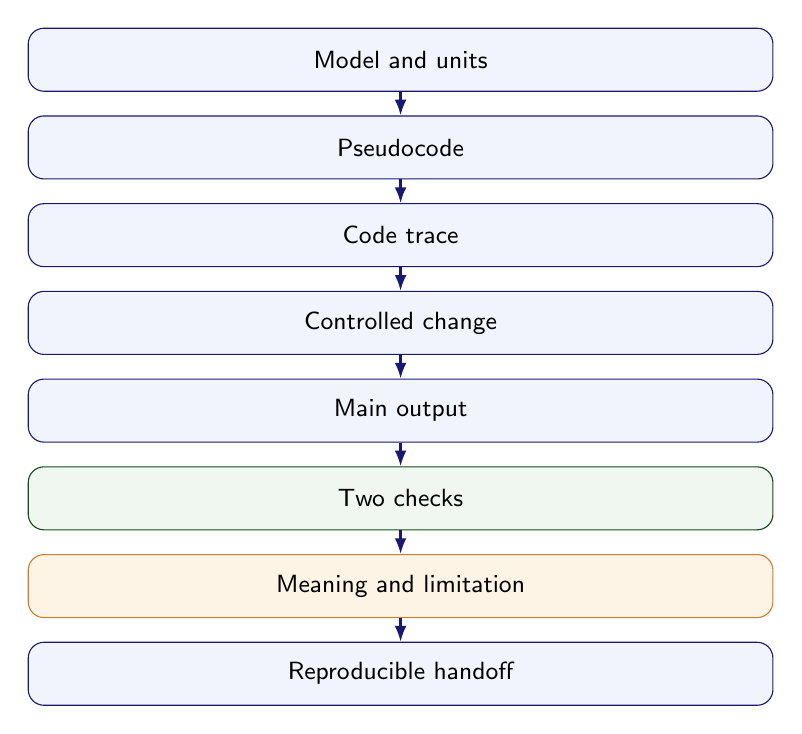
\begin{tikzpicture}[node distance=3mm,every node/.style={font=\small\sffamily,align=center},box/.style={draw=MidnightBlue,rounded corners=2mm,fill=RoyalBlue!7,minimum width=.78\linewidth,minimum height=8mm},check/.style={draw=ForestGreen!55!black,rounded corners=2mm,fill=ForestGreen!7,minimum width=.78\linewidth,minimum height=8mm},warn/.style={draw=BurntOrange!80!black,rounded corners=2mm,fill=BurntOrange!8,minimum width=.78\linewidth,minimum height=8mm},arrow/.style={-{Latex[length=2mm]},thick,MidnightBlue}]
\node[box] (m) {Model and units};
\node[box,below=of m] (p) {Pseudocode};
\node[box,below=of p] (c) {Code trace};
\node[box,below=of c] (chg) {Controlled change};
\node[box,below=of chg] (o) {Main output};
\node[check,below=of o] (v) {Two checks};
\node[warn,below=of v] (l) {Meaning and limitation};
\node[box,below=of l] (h) {Reproducible handoff};
\draw[arrow] (m)--(p);\draw[arrow] (p)--(c);\draw[arrow] (c)--(chg);\draw[arrow] (chg)--(o);\draw[arrow] (o)--(v);\draw[arrow] (v)--(l);\draw[arrow] (l)--(h);
\end{tikzpicture}
\end{center}
Read the sequence from top to bottom. The model and units prevent a silent change of physical meaning. The pseudocode makes the order inspectable. The code trace shows what the script actually computes. The main output answers the one question. The checks support specific claims. Meaning and limitation prevent overclaiming. The reproducible handoff lets another student repeat the sequence.
\section*{2. Keep the investigation bounded}
The capstone is a supported investigation rather than an open-ended research project. The scope below is the ordinary required route.
\begin{center}\small
\begin{tabular}{>{\raggedright\arraybackslash}p{.25\linewidth}>{\raggedright\arraybackslash}p{.62\linewidth}}
\toprule
\textbf{Evidence item} & \textbf{What the group must show}\\ \midrule
Physical question & One narrow question about a supplied or approved physical behaviour.\\
Controlled change & One parameter or assumption changes; all other important inputs are named as fixed.\\
Main output & One labelled graph or table that directly answers the question, with quantities, units, and cases.\\
Required check & The validation check agreed in the model and method plan.\\
Chosen check & A second check using genuinely different evidence or testing a different weakness.\\
Interpretation & One physical conclusion linked to the prediction.\\
Limitation & One numerical or model limitation that marks where the claim stops.\\
Handoff & Edited starter, inputs, settings, run order, clean-session record, and a short AI decision record.\\
\bottomrule
\end{tabular}
\end{center}
\begin{aibox}\textbf{Do not broaden the question at the last moment.} A second graph, an extra method, or an independent extension can be interesting, but it is not a substitute for a complete required evidence chain. Remove optional material if it hides the main output or the checks.\end{aibox}
\section*{3. Model first: variables and units}
Before showing MATLAB, state the physical picture, assumptions, and output. Every important code variable should map to a physical quantity and unit. Keep numerical settings visible because a timestep, grid, angle array, or reference value is part of the evidence.
\begin{center}\small
\begin{tabular}{>{\raggedright\arraybackslash}p{.24\linewidth}>{\raggedright\arraybackslash}p{.28\linewidth}>{\raggedright\arraybackslash}p{.36\linewidth}}
\toprule
\textbf{Record} & \textbf{Example name} & \textbf{Purpose}\\ \midrule
Question & range versus launch angle & identifies the physical output\\
Parameter & \texttt{v0\_mps} & changed or fixed input with unit m s$^{-1}$\\
Discretisation & \texttt{angle\_deg = 0:5:90} & finite set of model inputs\\
Method & parameter sweep & supplied computational recipe\\
Output & \texttt{range\_m} & main result with unit m\\
Check & 45 degree reference & known result or independent evidence\\
\bottomrule
\end{tabular}
\end{center}
The example track in the starter uses level landing without air drag:
\[
R(\theta)=\frac{v_0^2\sin(2\theta)}{g}.
\]
In words: horizontal range is launch speed squared, multiplied by the angle factor, divided by the gravitational acceleration. The supplied baseline uses $v_0=18\units{m\,s^{-1}}$ and the controlled modification uses $v_0=20\units{m\,s^{-1}}$, while $g=9.81\units{m\,s^{-2}}$ and the angle array remain fixed. The practical brief and starter use the same five canonical supplied tracks. Your approved track may use any one of these familiar models.
\begin{checkbox}\textbf{Prediction checkpoint.} Before running the modified case, state whether the main output should increase, decrease, change sign, approach a bound, or change shape. A prediction gives the final output a testable reference.\end{checkbox}
\section*{4. Pseudocode before code}
Use short plain-language steps. A teammate should be able to point to the job of each code block before seeing its MATLAB syntax.
\begin{enumerate}[nosep,leftmargin=6mm]
\item record the approved model, assumptions, inputs, and units;
\item calculate the baseline output with the supplied method;
\item change one parameter or assumption and keep the other inputs fixed;
\item calculate the modified output and choose one main graph or table;
\item run the required check and a different chosen check; and
\item interpret the pattern, state one limitation, and record the clean-session handoff.
\end{enumerate}
\begin{keybox}\textbf{Code-tracing prompt.} Choose one relevant line. What quantity does it represent? Which pseudocode step does it complete? What output would reveal a wrong sign, wrong unit, wrong index, or wrong array operation?\end{keybox}
\section*{5. A worked validation example}
For the supplied projectile track, the 45 degree result has a known form:
\[
R(45^\circ)=\frac{v_0^2}{g}.
\]
The script compares the calculated baseline value at 45 degrees with this reference. This is the required check for the default track. The chosen check uses a different relationship: the range curve should be symmetric, so $R(\theta)=R(90^\circ-\theta)$ for the chosen angle array. These are two genuinely different validation checks: the reference value tests agreement at one known point, while symmetry tests the shape of the whole modelled relationship. Two versions of the same comparison, such as repeating the endpoint check at two speeds or comparing the same curve at two resolutions, do not count as two different checks.
\Needspace{10\baselineskip}
\begin{lstlisting}[style=matlabstyle,caption={MATLAB code for the projectile baseline output and two genuinely different validation checks}]
range_m = v0_mps^2*sind(2*angle_deg)/g_mps2;
angle_45_index = find(angle_deg == 45,1);
reference_range_45_m = v0_mps^2/g_mps2;
reference_error_m = abs(range_m(angle_45_index)-reference_range_45_m);
symmetry_error_m = max(abs(range_m-fliplr(range_m)));
assert(reference_error_m < 1e-12)
assert(symmetry_error_m < 1e-12)
\end{lstlisting}
The first assertion tests agreement with a known value. The second checks a different structural property of the model. Both pass for the supplied baseline. Passing checks do not prove that the no-air-drag assumption is realistic; they support narrower claims about the calculation and the stated model.
\begin{checkbox}\textbf{Validation language.} Say what the evidence supports and what it does not establish. ``The code looks reasonable'' is not a validation argument; a value, bound, reference, residual, conservation relation, or clean rerun is concrete evidence.\end{checkbox}
\section*{6. Main output and physical meaning}
The main graph or table should answer the original question directly. Label the measured or modelled quantity, its unit, the baseline case, the modified case, and the changed parameter. State one pattern for the audience to notice before adding secondary detail.
For the projectile example, the modified speed increases the range at the same angle because the model contains $v_0^2$. The curve peaks near 45 degrees for the level-landing, no-drag model. A limitation is that the ideal model omits air resistance and therefore does not claim to predict a real projectile in every condition.
Keep two kinds of limitation separate:
\begin{itemize}[nosep,leftmargin=6mm]
\item numerical limitation: resolution, timestep, approximation, or reference comparison; and
\item model limitation: an idealisation such as no drag, constant parameters, or expected count rather than an individual random count.
\end{itemize}
\section*{Guided extension}
After the required output is clear, a group may use supplied evidence from a second numerical resolution, a second familiar method, or a second parameter range to deepen the discussion. Treat this as supporting evidence, not as a replacement for the one main output and two checks.
\section*{Optional extension}
An independent extension or deeper method comparison may be added after the complete required handoff. It is optional and not required for ordinary completion; removing it must leave the model, output, validation, interpretation, and reproducibility pathway intact.
\Needspace{19\baselineskip}
\section*{7. Defence and responsible AI evidence}
The shared group result does not remove the individual explanation. Each member should trace one relevant code section, explain its physical meaning, and answer one parameter-change or validation follow-up. The lecturer keeps a rotation ledger with one entry per student: complete one defence for every group member before assigning a second. Mark an absence as pending and add a make-up entry when the deferred defence is completed.
\begin{aibox}\textbf{AI decision record.} Write one short record: what assistance was requested; what was accepted, modified, or rejected; why; and which independent checks supported the final claim. Do not submit a complete chat transcript, and do not use an AI-detection score as evidence of learning or misconduct.\end{aibox}
\section*{8. Reproducible handoff}
Another student should be able to start from a fresh MATLAB R2025a-or-later session and regenerate the main output and both checks. The handoff must record:
\begin{enumerate}[nosep,leftmargin=6mm]
\item the edited starter Live Script, required input files, parameter values, assumptions, units, and numerical settings;
\item the run order and MATLAB release;
\item the main output plus both checks, numerical evidence, physical conclusion, and one limitation; and
\item the concise AI decision record and individual defence entries, including any pending absence or make-up record.
\end{enumerate}
Run the final script from the top in a fresh session before marking the evidence final in the submission record. Keep the edited script and inputs together. If a dependency is not base MATLAB, name it explicitly rather than leaving another student to guess.
\begin{keybox}\textbf{Final evidence state.} Mark the evidence \emph{final in the submission record} only after the clean rerun reproduces the main output and both checks, the handoff record is complete, and every group member has a recorded defence entry or a clearly pending make-up entry.\end{keybox}
\begin{keybox}\textbf{Preparation for the presentation.} Open the starter script, select the approved track, read the model and units aloud, make the prediction, trace one code line, and locate both validation results. Bring the editable script and handoff checklist to the group review.\end{keybox}
\section*{Three takeaways}
\begin{enumerate}[nosep,leftmargin=6mm]
\item A bounded question makes a computational result easier to interpret and defend.
\item Two checks are useful only when they test different claims or weaknesses.
\item Reproducibility is part of the scientific result: another student should know what to open, run, check, and conclude.
\end{enumerate}
\end{document}
